\subsection{cluster finder}

cluster finder首先在基于slow simulator产生的数据上进行测试。计划是当用simulator的数据cluster finder可以得到比较好表现之后再用真实数据进行测试。在本小节当中将会对cluster finder的工作方式以及初步的测试结果进行讨论。

cluster finder的工作流程如图\ref{fig:Cluster_Finder_work_flow}所示。首先要做的是从各个不同的读出条组的读出信息当中进行一维cluster的寻找。因为sTGC的结构设计上是多个一维读出的室组合而成最后的模组,所以得到了一维cluster的信息之后要做的就是将一维cluster重建成对应的二维cluster信息,并且因为是从一维cluster重建二维的cluster,会产生大量的ghost hit,如何对ghost hit进行排除将会在后文当中进行详细的介绍。当这些步骤全部完成之后剩下的cluster我们认为就是探测器最后探测到的真实的hit,并将这些信息储存下来。在本小节中会对整个cluster finder的工作方式进行介绍。

\begin{figure}[htb]
    \begin{center}
    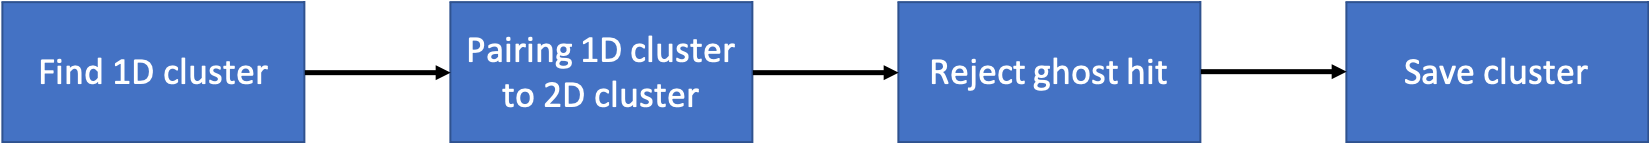
\includegraphics[width=0.7\textwidth,clip]{figures/Chapter3/Cluster_Finder_work_flow.png}
    \end{center}
    \caption[cluster finder工作流程示意图]{cluster finder工作流程示意图}
    \label{fig:Cluster_Finder_work_flow}
\end{figure}

在介绍cluster finder的工作流程之前,首先要讨论当一个带电粒子击中sTGC的时候会发生什么以及会留下哪些信息被我们收集到。

一个sTGC的模组结构和工作原理已经在\ref{chap:3_2}小节中进行了介绍,当一个带电粒子击中sTGC模组的时候会在X、Y和垂直于对角线的方向上分别产生信号并被读出。我们能直接得到的只有每个cluster在这三个方向上的投影,即当产生一个cluster的时候这个cluster会对应三个方向上的信号读出。当同时击中的cluster大于两个的时候会产生ghost hit问题。当有n个cluster同时击中sTGC的一个模组的时候,会在每个方向上产生n个一维的cluster,这样如果只有二维的信息进行配对,我们可能重建出来${\rm n^2}$个二维的cluster信息,相比于真实的cluster数目多重建出了${\rm n^2}-1$个cluster。这些多出来的cluster即为ghost hit。为了解决这个问题,沿对角线方向的读出条被引入来减少ghost hit的数目。这样多出了一个维度的信息来对cluster的数目进行限制。图\ref{fig:Ghost_hit}展示了当有四个cluster同时击中的时候,所对应的ghost hit的位置和沿对角线方向的cluster如何来对ghost hit进行限制。

如图\ref{fig:Reject_Ghost_Hit}所示,当一个cluster落在沿对角线方向上的一个读出条的时候,因为读出条是沿着平行于二四象限的角平分线方向,其两个长边对应的方程分别为$y = -x+a_1$以及$y = -x+a_2$。即落在这个范围内的点(x,y),应该满足$ a_1 < x+y < a_2 $ 的条件。这样我们可以得到每个沿着对角线方向上的读出条对应的截距的上下限范围。而对于在对角线上侧和下侧的点,可以通过$x>y$和$x < y$来进行区分。这样沿着对角线方向的坐标被引入用来限制ghost hit。

\begin{figure}[htb]
    \centering
    \begin{subfigure}[b]{0.45\textwidth}
        \centering
        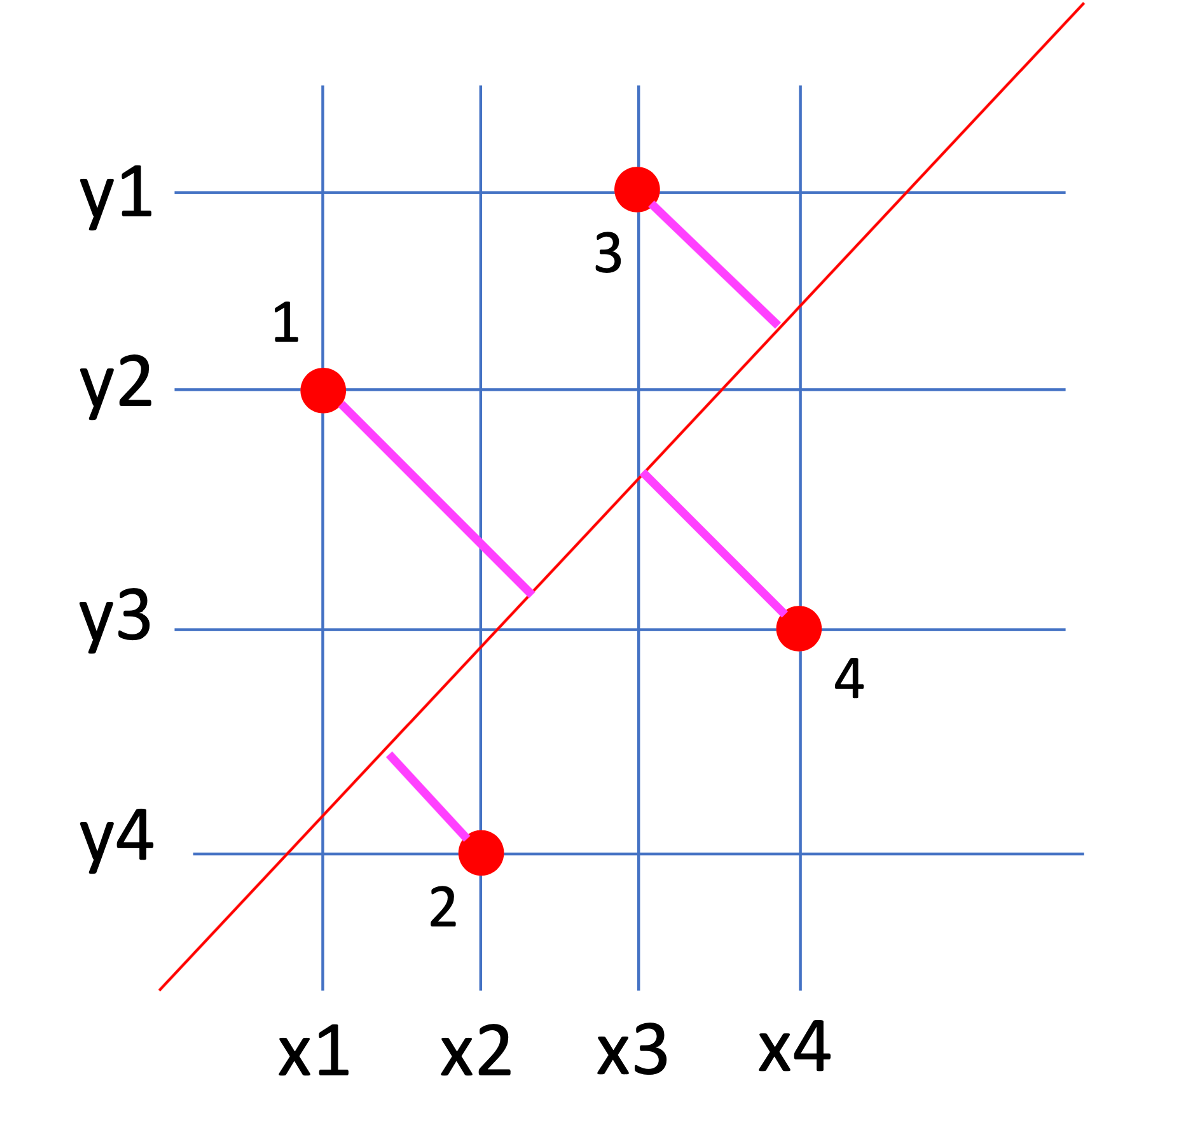
\includegraphics[width=\textwidth,clip]{figures/Chapter3/Ghost_hit.png}
        \caption{}
        \label{fig:Ghost_hit}
    \end{subfigure}
    \hfill
    \begin{subfigure}[b]{0.45\textwidth}
        \centering
        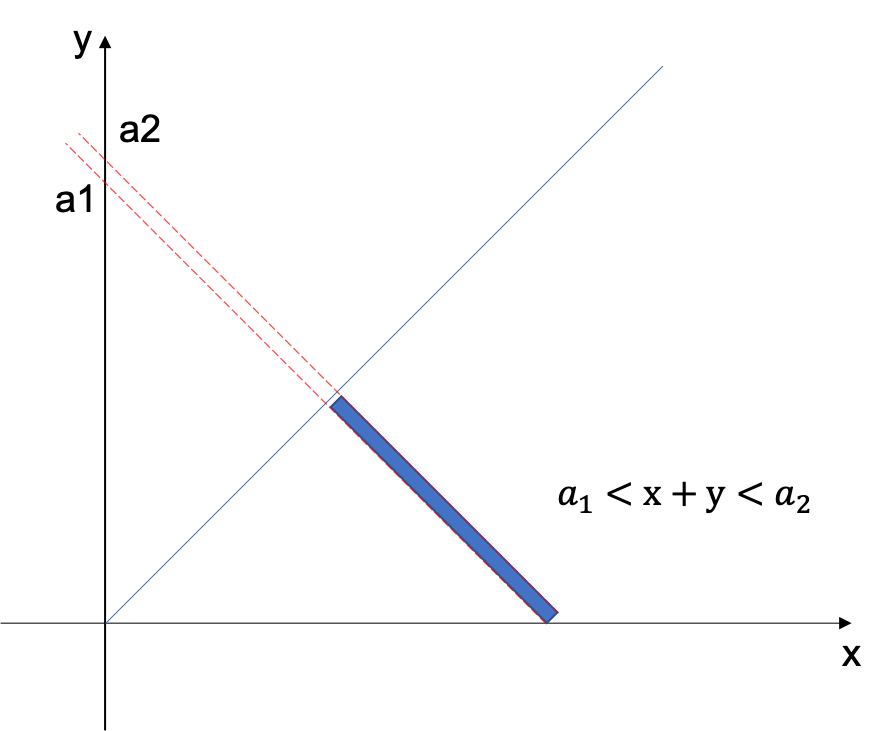
\includegraphics[width=\textwidth,clip]{figures/Chapter3/Reject_Ghost_Hit.png}
        \caption{}
        \label{fig:Reject_Ghost_Hit}
    \end{subfigure}
    \caption[Ghost hit原理及排除方法示意图]{\ref{fig:Ghost_hit}为当有四个cluster击中sTGC时信号读出示意图。1、2、3和4分别为四个cluster的击中位置,$x_i$和$y_i$分别为四个cluster在X和Y方向上重建出来的cluster的位置。紫红色线显示了四个cluster在沿着对角线方向上的读出条组的cluster读出。\ref{fig:Reject_Ghost_Hit}为击中一个沿对角线方向的读出条的对应的截距范围示意图。$a_1$以及$a_2$分别为图中读出条对应的截距上下限}
       \label{fig:Ghost_Hit_plots}
\end{figure}

同时,因为在沿着每个方向上的读出条组被分成了三段,这样两两组合就会组成8个读出条组,而每个读出条组都会有自己独特的边界条件,如图\ref{fig:Strip_Group}所示。当一个(x,y)的组合不满足这8个组的任何一个组的边界条件的时候,也可以认为这个组合来源于一个ghost hit。

\begin{figure}[htb]
    \begin{center}
    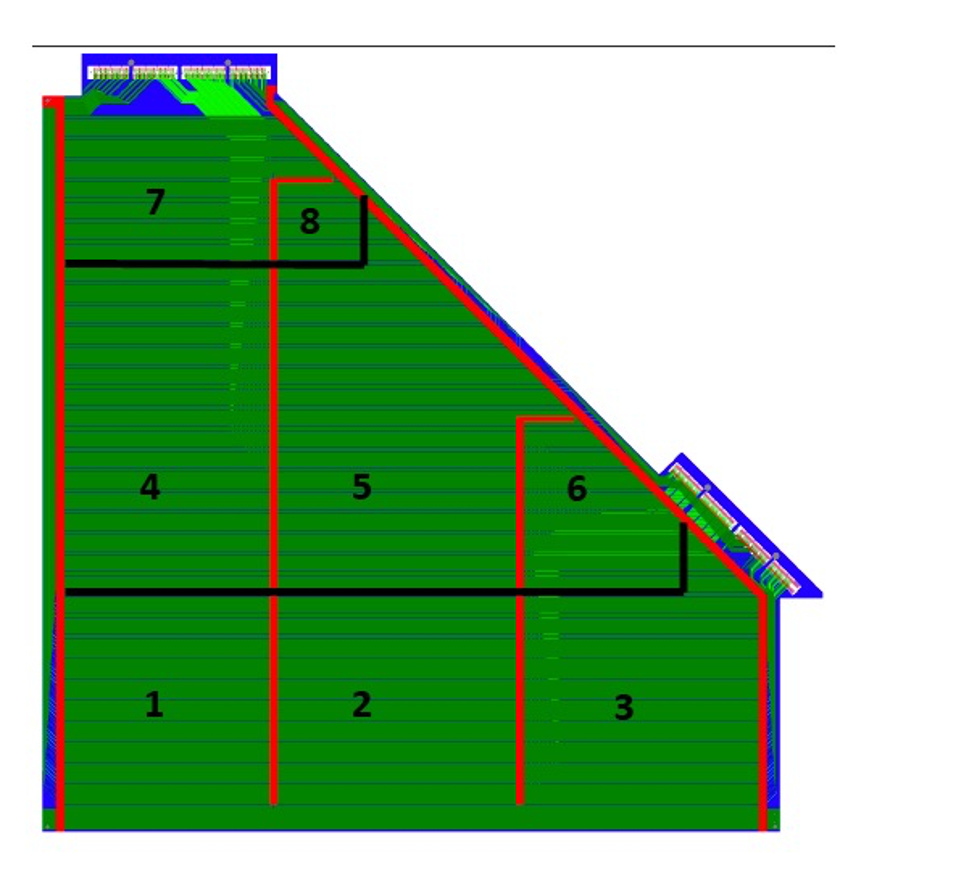
\includegraphics[width=0.7\textwidth,clip]{figures/Chapter3/Strip_Group.png}
    \end{center}
    \caption[读出条组示意图]{读出条组示意图。因为在每个方向上的读出条被分成了三个读出条组,这样在二维的平面上读出条一共被分成8个读出条组}
    \label{fig:Strip_Group}
\end{figure}

如\ref{chap:3_2}中提到的一样,cluster finder采用电荷重心法来重建cluster的位置,那么对于cluster finder来说,首先要能做到的就是找到一个cluster。
在slow simulator和最后安装在STAR上的探测器当中,使用的电子学和原型机测试时不同,为VMM电子学。VMM和TPX电子学有一个显著的不同就是它是一种峰值读出的电子学,在一个感应信号产生的过程中VMM只会记录整个电信号峰值所对应的PDO(作用和TPX电子学当中的ADC相同)和时间。所以说并不用像TPX电子学一样对单读出条的信号的持续时间进行研究。当VMM读出信号的时候即意味着有一个信号波形被其接收到。

当一个读出条组读到信号之后可以将所有读出条按照读出条编号的顺序排列,就可以得到沿着读出条方向投影的每个读出条上的电荷分布。如图\ref{fig:ADC_Group_Projection}所示。可以看到每个cluster在沿着读出条方向上的投影都留下了一个峰的信号结构。有一个很自然的假设就是当读出条离发生电离的位置越远的时候在该读出条上面产生的感应信号的幅度越小,这也是电荷重心法确定位置的基础,也在宇宙线测试当中被证实。整个寻找cluster的算法也是基于这个假设。步骤如下:
\begin{itemize}
    \item[1.] 将所有的读出条序号和对应ADC的值一一对应存放到库中。
    \item[2.] 将所有的读出条按照ADC大小排列,找到ADC最大的读出条以及其序号,读出条序号记为i。
    \item[3.] 以ADC最大的读出条为起点,读取第(i-1)根和第(i+1)根读出条的ADC信息。
    \item[4.] 当${\rm ADC_{i-1} < ADC_{i}}$时继续读取第(i-2)根读出条的ADC信息。 

              当${\rm ADC_{i-n} > ADC_{i-(n-1)}}$或者${\rm ADC_{i-n} = 0}$时停止,并记录n。
    \item[5.] 当${\rm ADC_{i+1} < ADC_{i}}$时继续读取第(i+2)根读出条的ADC信息。

              当${\rm ADC_{i+m} > ADC_{i+(m-1)}}$或者${\rm ADC_{i-m} = 0}$时停止,并记录m。
    \item[6.] 当$(m+n)-1 >= 3$时认为找到一个cluster,利用式\ref{eq:center_of_gravity}计算cluster位置并将第i+(n-1)至i+(m-1)之间的读出条信息从库中移除。之后重复2-5步。直到$(m+n)-1 < 3$
    \item[7.] 当$(m+n)-1 < 3$时停止寻找cluster,流程结束。
\end{itemize}
\begin{figure}[htb]
    \begin{center}
    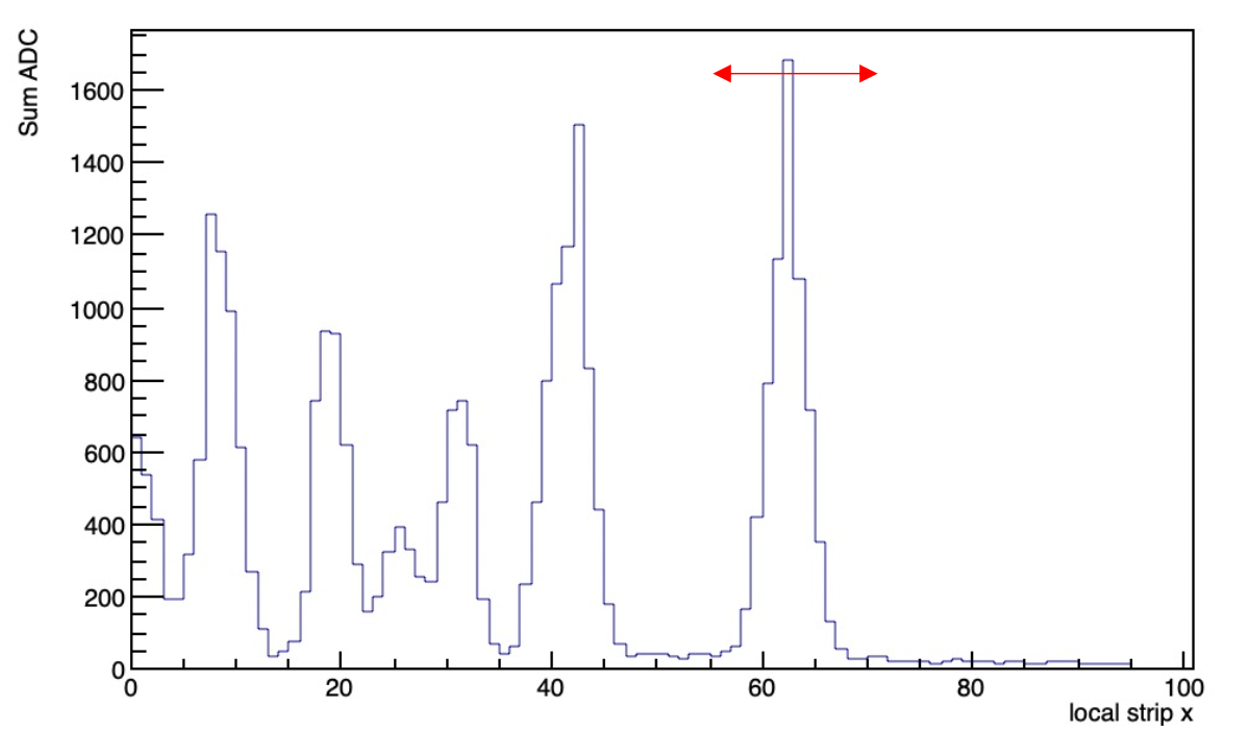
\includegraphics[width=0.7\textwidth,clip]{figures/Chapter3/ADC_Group_Projection.png}
    \end{center}
    \caption[一个读出条组在一个事例当中的电荷分布]{一个读出条组在一个事例当中的电荷分布,x轴为在当前读出条组当中的编号,y轴为当前事例在此读出条上ADC的值。}
    \label{fig:ADC_Group_Projection}
\end{figure}

经过上述的步骤之后,从每个读出条组筛选出cluster信号并且储存起来。一维cluster的重建结束。这样我们就可以得到cluster们在X、Y和垂直于对角线方向上的坐标。下一步要做的就是将这些一维cluster重建成二维cluster。将X、Y方向上的坐标进行配对,得到一组坐标(x,y)。首先判断(x,y)是否满足八个读出条组的边界条件,如果不满足的话即认为是一个ghost hit,将其抛弃。再根据x和y的大小关系以及x+y的值去寻找对应的沿对角线方向上的读出条是否有一维cluster的值落在了相同的读出条范围内,如果有的话,则认为找到一个真实的cluster,并保存下来。如果没有则认为此(x,y)对为ghost hit,将其抛弃。

结束对ghost hit的排除之后剩下的cluster便是由cluster finder重建出来的cluster的位置。对于每个模组来说,当单独处理本模组内的cluster的时候可以认为是在第一象限内进行处理,在处理完之后再根据不同模组的位置信息cluster的局部坐标进行坐标转换成为全局坐标。从第一象限到其他几个象限的坐标转换关系如表\ref{tab:Coordinate_conversion}所示。其中shift为位于三四象限的两个sTGC模组向外平移的距离。需要注意的是,在slow simulator中假设原点位于一二象限两个探测器重合的角的位置,在实际的处理当中整个X-Y平面的原点应该位于束流管的中心位置,和slow simulator的数据有出入。同时因为在整个探测器的下部需要支撑结构的问题,位于三四象限的两个探测器分别向外平移了一段距离。这都是在坐标变换的时候需要注意的地方。

\begin{table}[h!]
    \centering
    \caption{sTGC位于不同象限的模组局部坐标到全局坐标的转换关系}
    \label{tab:Coordinate_conversion}
    \begin{tabularx}{0.9\textwidth} {| >{\centering\arraybackslash}X |>{\centering\arraybackslash}X |>{\centering\arraybackslash}X |>{\centering\arraybackslash}X |}
        \hline
        第一象限 & 第二象限 &  第三象限 &  第四象限\\
        \hline
        $(x,y) \rightarrow (x,y)$& $(x,y) \rightarrow (y,x)$ & $(x,y) \rightarrow (-x-shift,-y)$ & $(x,y) \rightarrow (-y,x+shift)$\\
        \hline
    \end{tabularx}
\end{table}

在cluster finder的初期测试当中是利用slow simulator产生的数据进行测试,在STAR的run22当中,前向窄隙室探测器被正式安装到了STAR上,sTGC软件组也在进行将cluster finder整合进STAR的软件框架当中的工作。之后介绍的结果为前期测试当中基于模拟数据的测试结果。

在测试的数据当中每个event当中产生10个cluster,在数据产生之后由cluster finder进行重建并且和模拟的cluster位置进行比较,从而确定重建效率和重建本身带来的分辨率(Resolution)。

首先被研究的是在一维上cluster 重建的分辨率。在初期的测试中发现cluster finder重建出来的cluster的分辨率很差,在X和Y的两个方向上约为300${\rm \mu m}$,远超100 \mum ,如图\ref{fig:Resolution_1}所示。如果cluster finder本身会带来这么大的位置分辨会严重影响整个探测器的表现。后来经过排查,产生如此大的位置分辨的原因来源于slow simulator本身的问题。

在早期版本的slow simulator当中,对于每个读出条的电荷响应通过如下步骤模拟:
\begin{itemize}
    \item[1.] 产生cluster的位置,记为$x_0$
    \item[2.] 以1mm为步长,以$x_0$为原点从高斯分布当中sample每个strip的电荷分布,当两步在同一个strip内的时候将值相加。
\end{itemize}
这其中第二步就带来了问题,在slow simulator当中,每两个读出条之间的间隔为3.2mm,这样就导致对于每个读出条来说,并不是每一个读出条都会被均匀的sample相同的步数,如图\ref{fig:Sample_step}所示。这样使得对于不同的读出条来说在sample的时候的权重并不完全相同,这导致在用电荷重心法重建坐标的时候有一个很大的误差。当这个问题被修正以后出现了新的问题,在X和Y方向当中$\delta_{x(y)}$分布都出现多峰结构,但是每个峰自己的宽度大约为100\mum ,见图\ref{fig:Resolution_2}以及\ref{fig:Resolution_3}。这意味着在某个地方出现了整体的坐标偏移。在随后的debug过程中导致这个问题的原因也被发现。
\begin{figure}[htb]
    \begin{center}
    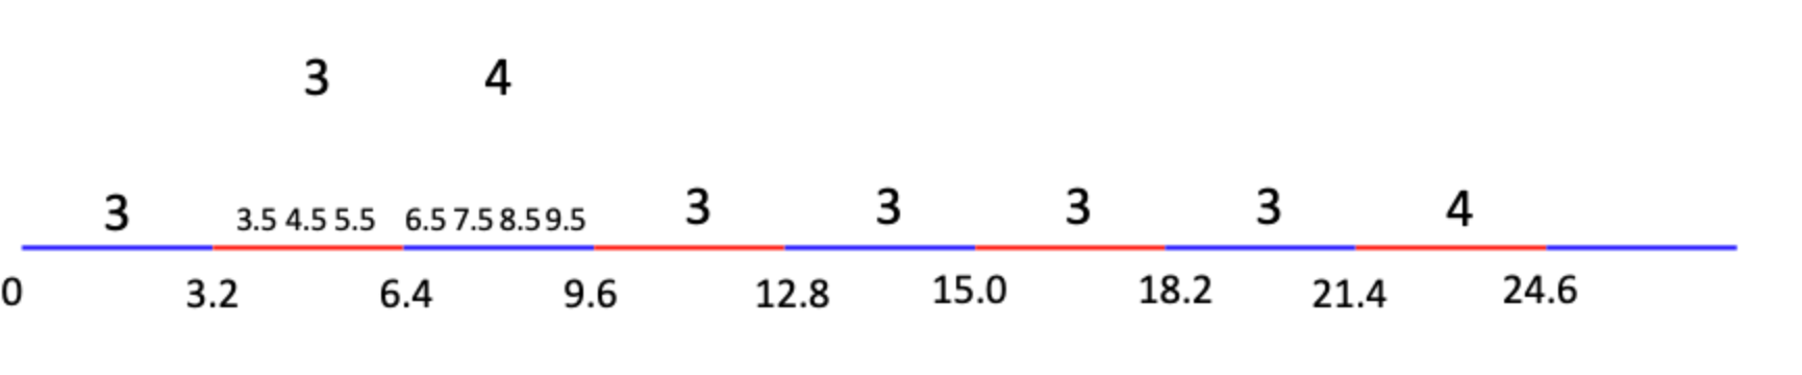
\includegraphics[width=0.7\textwidth,clip]{figures/Chapter3/Sample_step.png}
    \end{center}
    \caption[步长为1mm的时候每个读出条内sample点的个数]{步长为1的时候每个读出条内sample点的个数。红色蓝色粗线示意不同的读出条,宽度为3.2mm,读出条上方数字为每个读出条内sample点的个数。右起第二和右起第三读出条上面的数字为每一步sample的位置}
    \label{fig:Sample_step}
\end{figure}

当fit单独的峰的时候我们发现在X方向上的两个偏离原点的峰中心值分别为${\rm \pm 0.8 mm}$,在Y方向上两个峰的中心值分别为${\rm \pm 0.25 mm}$。在X方向的的差值为1/4个读出条的宽度(在slow simulator当中一个读出条的宽度被设置为3.2mm,即实际中一个读出条(2.7mm)加一条缝(0.5mm)的宽度)。造成这个偏差的原因是三四两个象限当中的模组相对于原点应该分别向X轴的正负方向平移了101.6mm,为31.75个读出条的的宽度,但是在设置这两个模组的局部坐标的时候依旧是从0开始,这样在坐标转换过程当中会造成1/4个读出条宽度的错位,这是在X方向上偏离0的两个峰的来源。在Y方向上的两个峰的来源也是来源于0点的设置问题,在一开始的设置中原点是第一个读出条的边界,而在计算位置的时候默认原点从第一个读出条往外半个缝的位置为0点,这就导致了有半个缝宽度的偏移,即0.25mm。这就是这两个方向上多峰结构的产生原因。这个问题在更新slow simulator和cluster finder之后被解决。

当sample步长和坐标对齐问题之后,cluster finder重建的分辨率可以达到100\mum 左右,满足对cluster fidner最初的设计要求。

\begin{figure}[htb]
    \centering
    \begin{subfigure}[b]{0.24\textwidth}
        \centering
        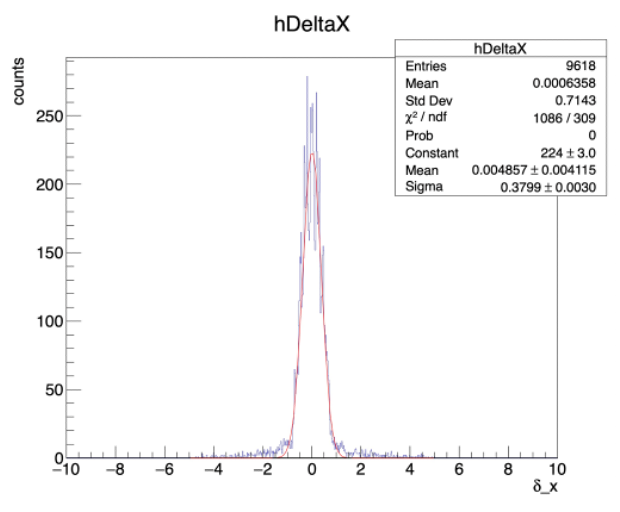
\includegraphics[width=\textwidth,clip]{figures/Chapter3/Resolution_1.png}
        \caption{}
        \label{fig:Resolution_1}
    \end{subfigure}
    \begin{subfigure}[b]{0.24\textwidth}
        \centering
        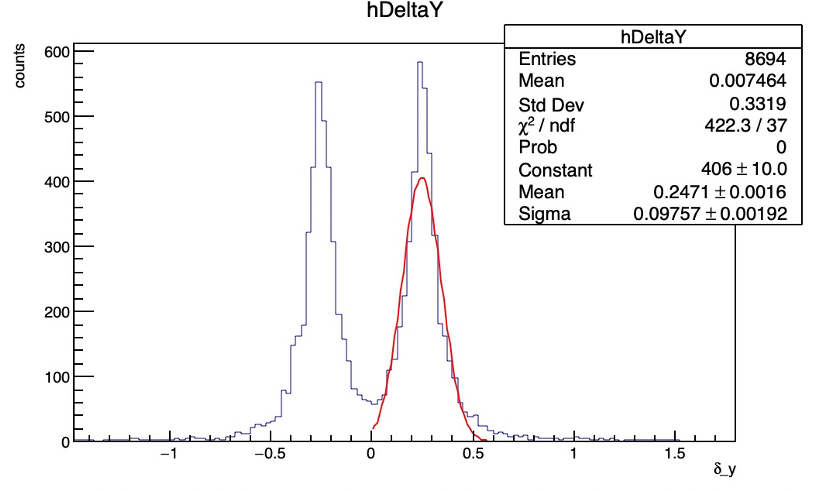
\includegraphics[width=\textwidth,clip]{figures/Chapter3/Resolution_2.png}
        \caption{}
        \label{fig:Resolution_2}
    \end{subfigure}
    \begin{subfigure}[b]{0.24\textwidth}
        \centering
        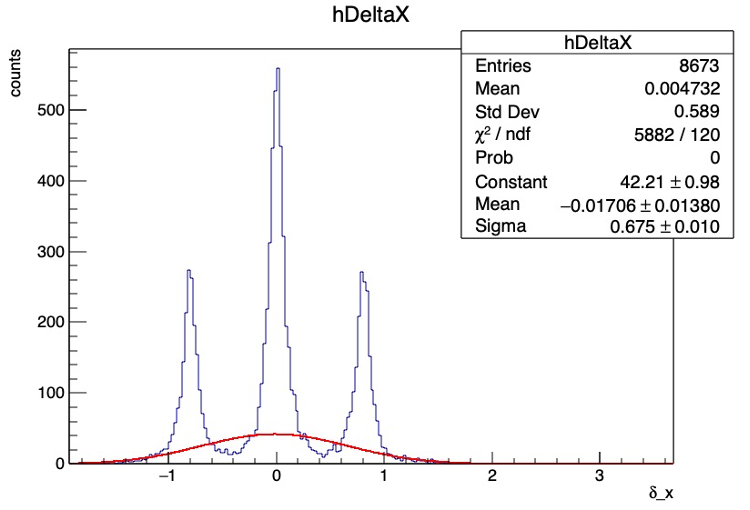
\includegraphics[width=\textwidth,clip]{figures/Chapter3/Resolution_3.png}
        \caption{}
        \label{fig:Resolution_3}
    \end{subfigure}
    \begin{subfigure}[b]{0.24\textwidth}
        \centering
        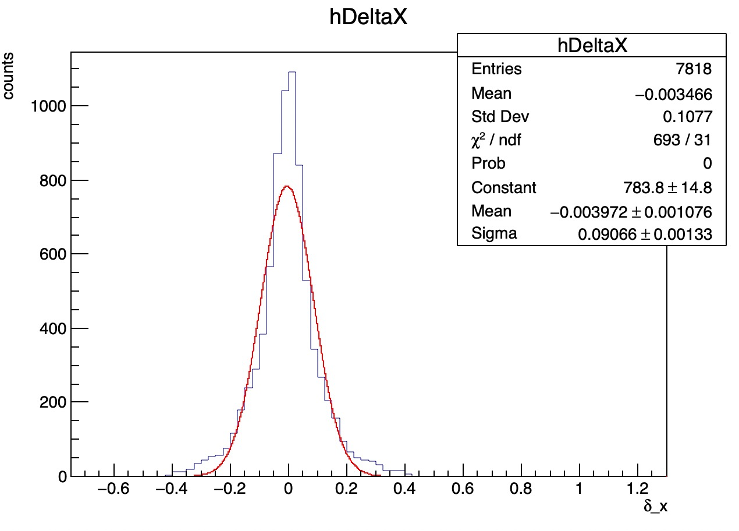
\includegraphics[width=\textwidth,clip]{figures/Chapter3/Resolution_4.png}
        \caption{}
        \label{fig:Resolution_4}
    \end{subfigure}
    \caption[Cluster finder 重建分辨率]{\ref{fig:Resolution_1}为sample步长为1的时候的一维重建分辨率。\ref{fig:Resolution_2}为修改步长后Y方向上的分辨率。\ref{fig:Resolution_3}为修改步长后X方向上的分辨率,\ref{fig:Resolution_4}为调整坐标对齐之后的分辨率}
       \label{fig:Ghost_Hit_plots}
\end{figure}

当分辨率达到要求之后开始对重建的效率进行测试,当cluster finder重建出来cluster的位置之后与slow simulator产生的cluster位置进行对比,当重建出来的cluster和模拟产生的cluster位置足够小的时候认为成功的重建出来一个cluster。通过这种方式可以计算重建的效率,重建效率的定义式如下:
\begin{equation}
    \epsilon = \frac{n_{r<R}}{n_{MC}}
\end{equation}
\begin{equation}
    r = \sqrt{(x^2-x^{\prime})^2 + (y^2-y^{\prime})^2}
\end{equation}

其中r为重建的cluster和模拟的cluster之间的距离,R为判断是否重建出来cluster的判选条件。(x,y)和${\rm(x^{\prime},y^{\prime})}$分别为模拟和重建的cluster的坐标。在探测器测试当中探测器的探测效率为97\%,则我们期望的经过三层组合之后的cluster重建效率应为90\%左右。在最新版本的cluster finder当中重建效率可以达到80\%左右,表现有待进一步提升。其主要问题是来源于对打在探测器边缘和读出条组边缘的cluster重建效率较低。对cluster finder的进一步测试和表现的改善的工作正在进行当中。